\documentclass[border=5pt]{standalone}
\usepackage{graphicx}
\usepackage{tikz}
\usetikzlibrary{shapes,snakes}
\usetikzlibrary{arrows.meta}
\usetikzlibrary{decorations}


%\renewcommand\familydefault{\sfdefault}

\begin{document}
\begin{tikzpicture}[]


\node[] at (10,16.5) (p1) {};
\node[anchor=south] at (p1) () {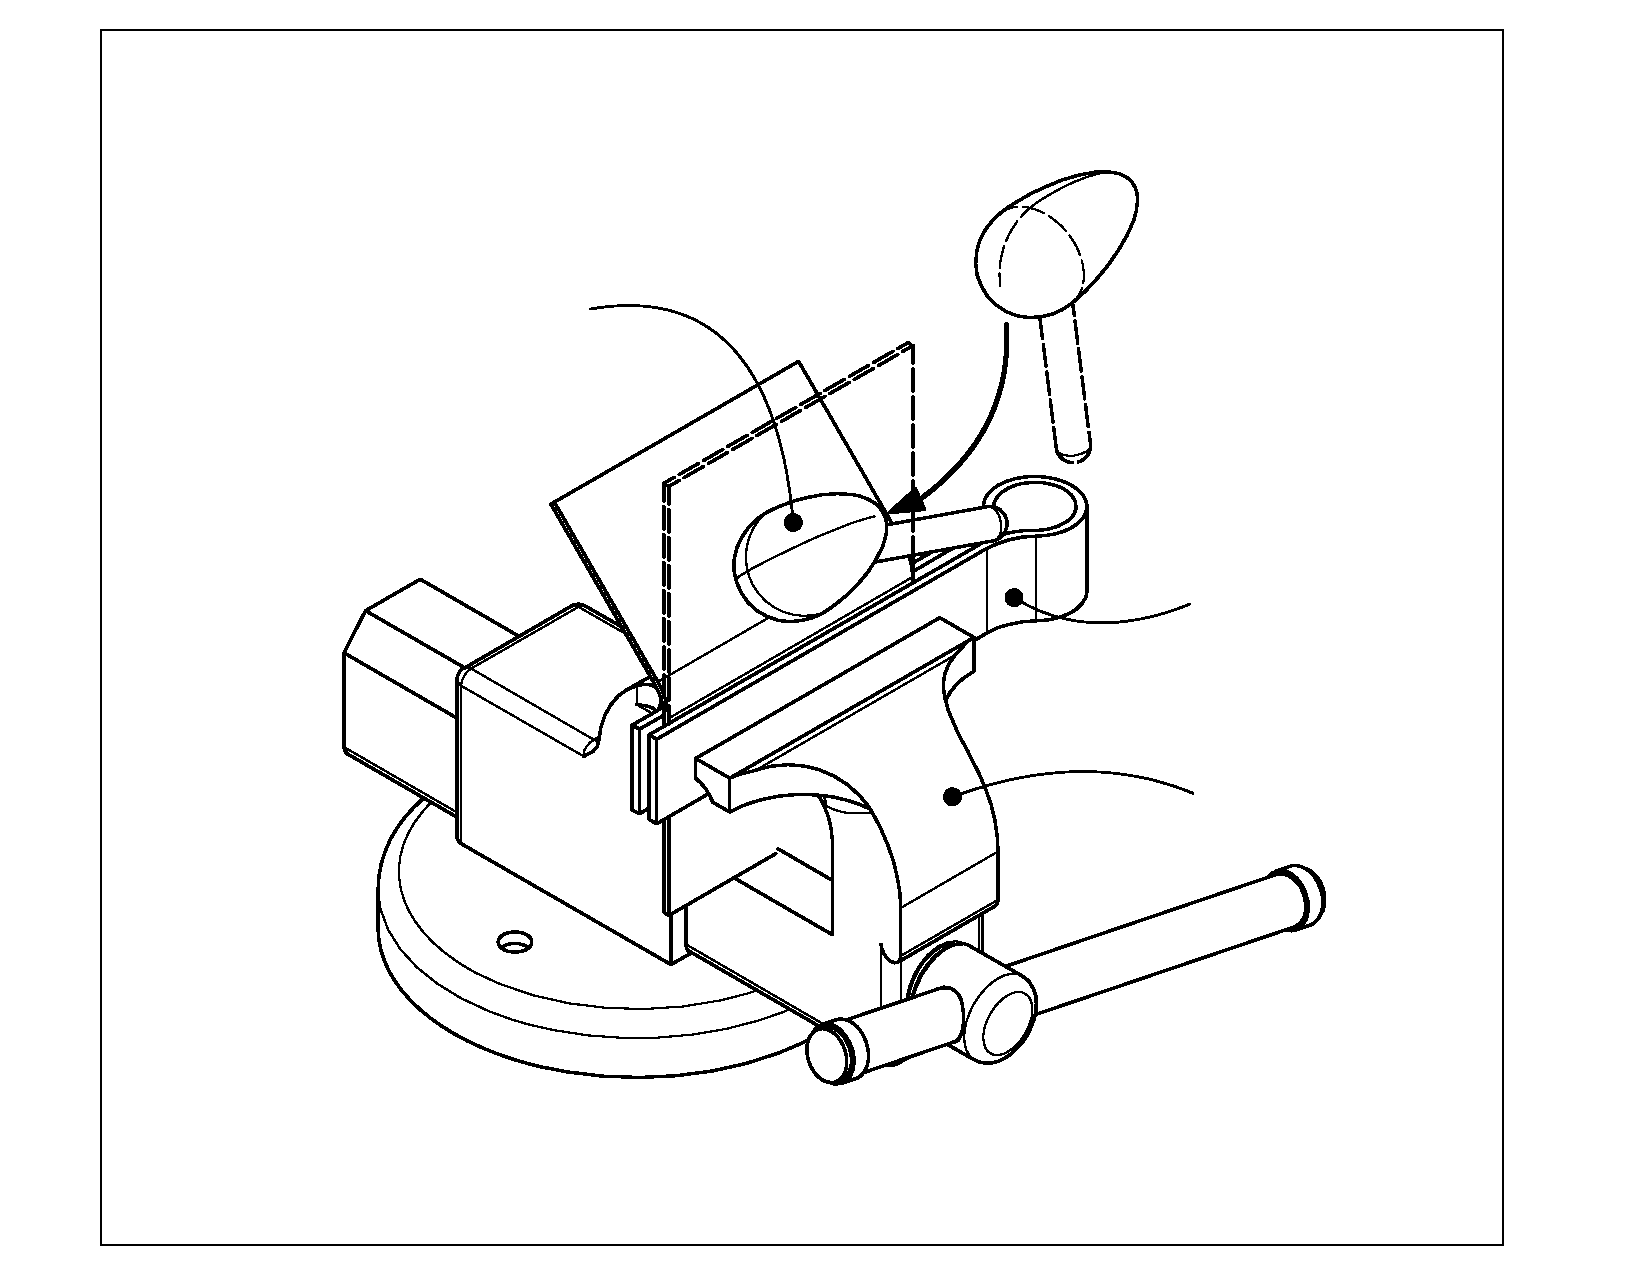
\includegraphics[trim={3cm 1cm 3cm 1cm },clip,width=6cm]{Images/DrawingsV3/FoldingTechDrawing.pdf}};
\node[anchor=north] at (p1) {(a)};
%
\node[] at (16.5,16.5) (p2) {};
\node[anchor=south] at (p2) () {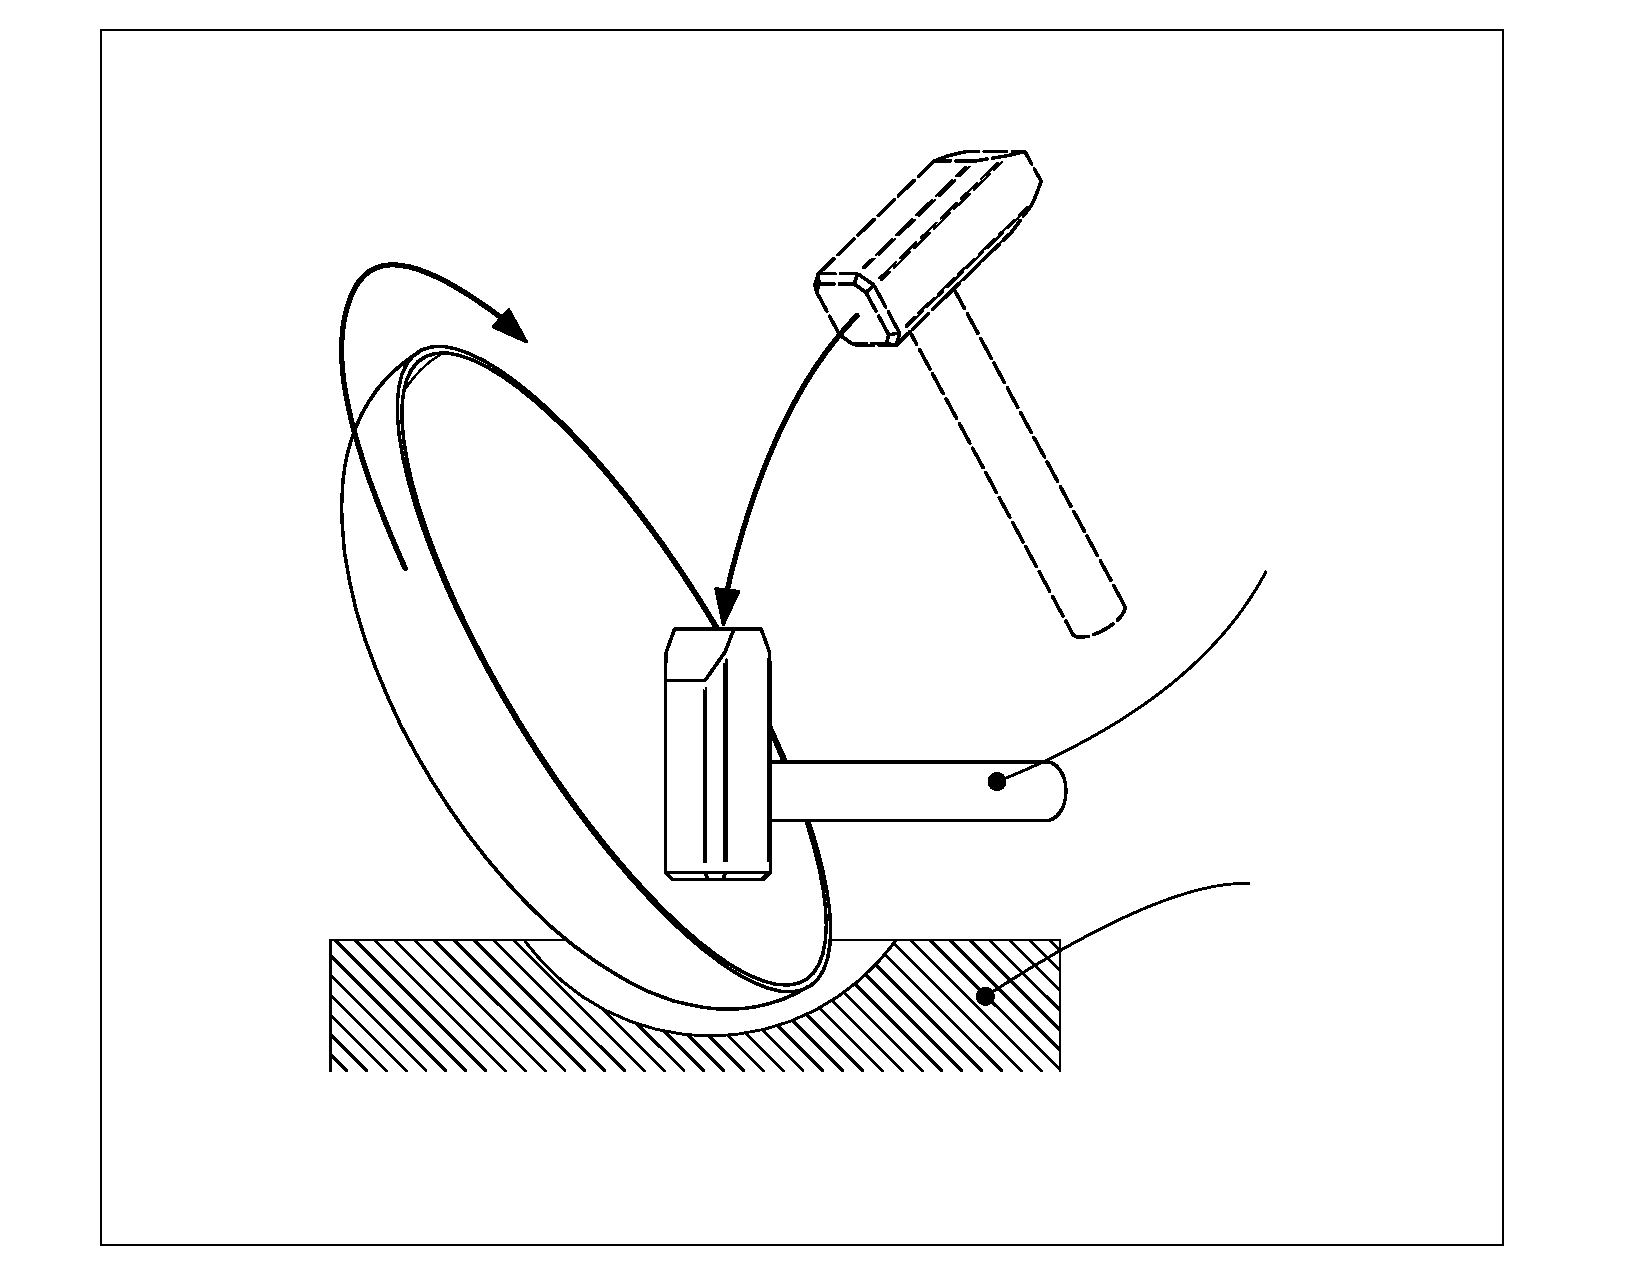
\includegraphics[trim={3cm 1cm 3cm 1cm },clip,width=6cm]{Images/DrawingsV3/HollowingTechDrawing.pdf}};
\node[anchor=north] at (p2) {(b)};
%
\node[] at (16.5,10) (p3) {};
\node[anchor=south] at (p3) () {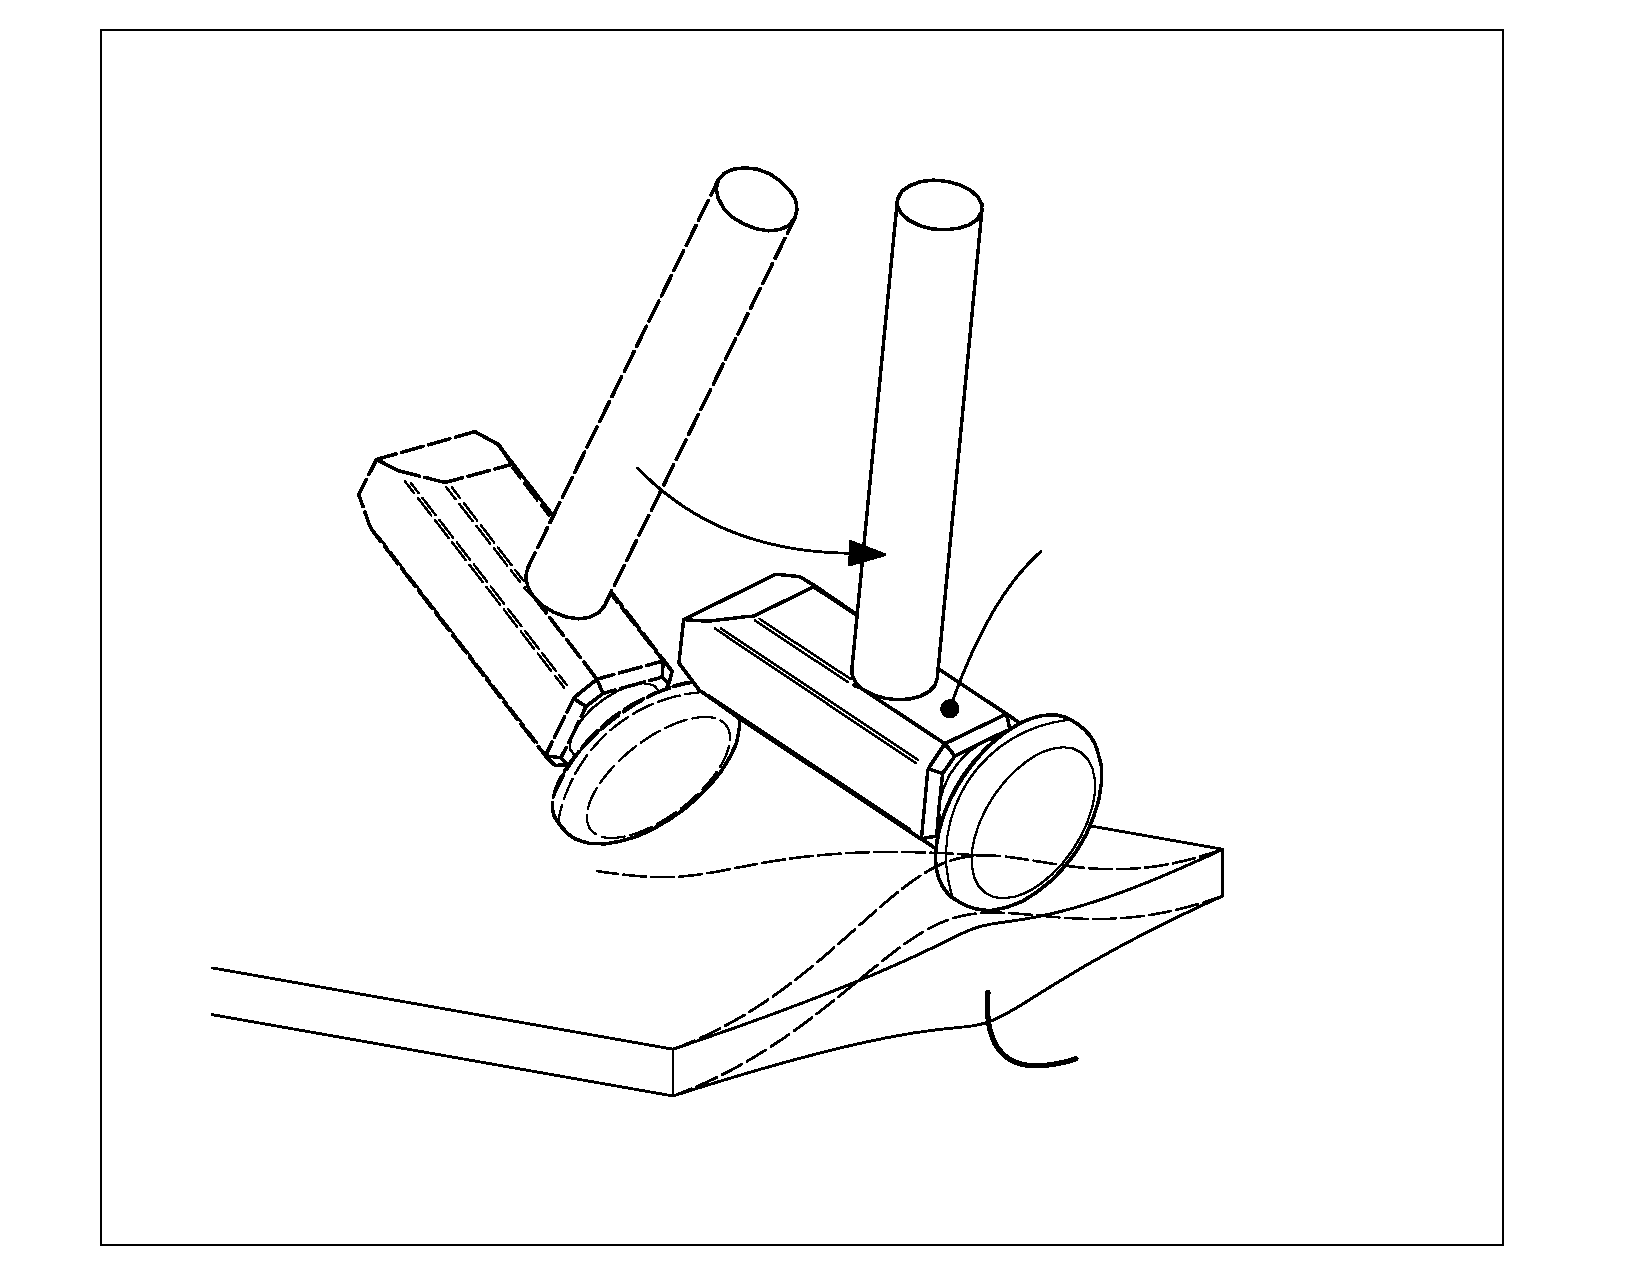
\includegraphics[trim={3cm 1cm 3cm 1cm },clip,width=6cm]{Images/DrawingsV3/ThickneingTechDrawing.pdf}};
\node[anchor=north] at (p3) {(d)};
%
\node[] at (10,10) (p4) {};
\node[anchor=south] at (p4) () {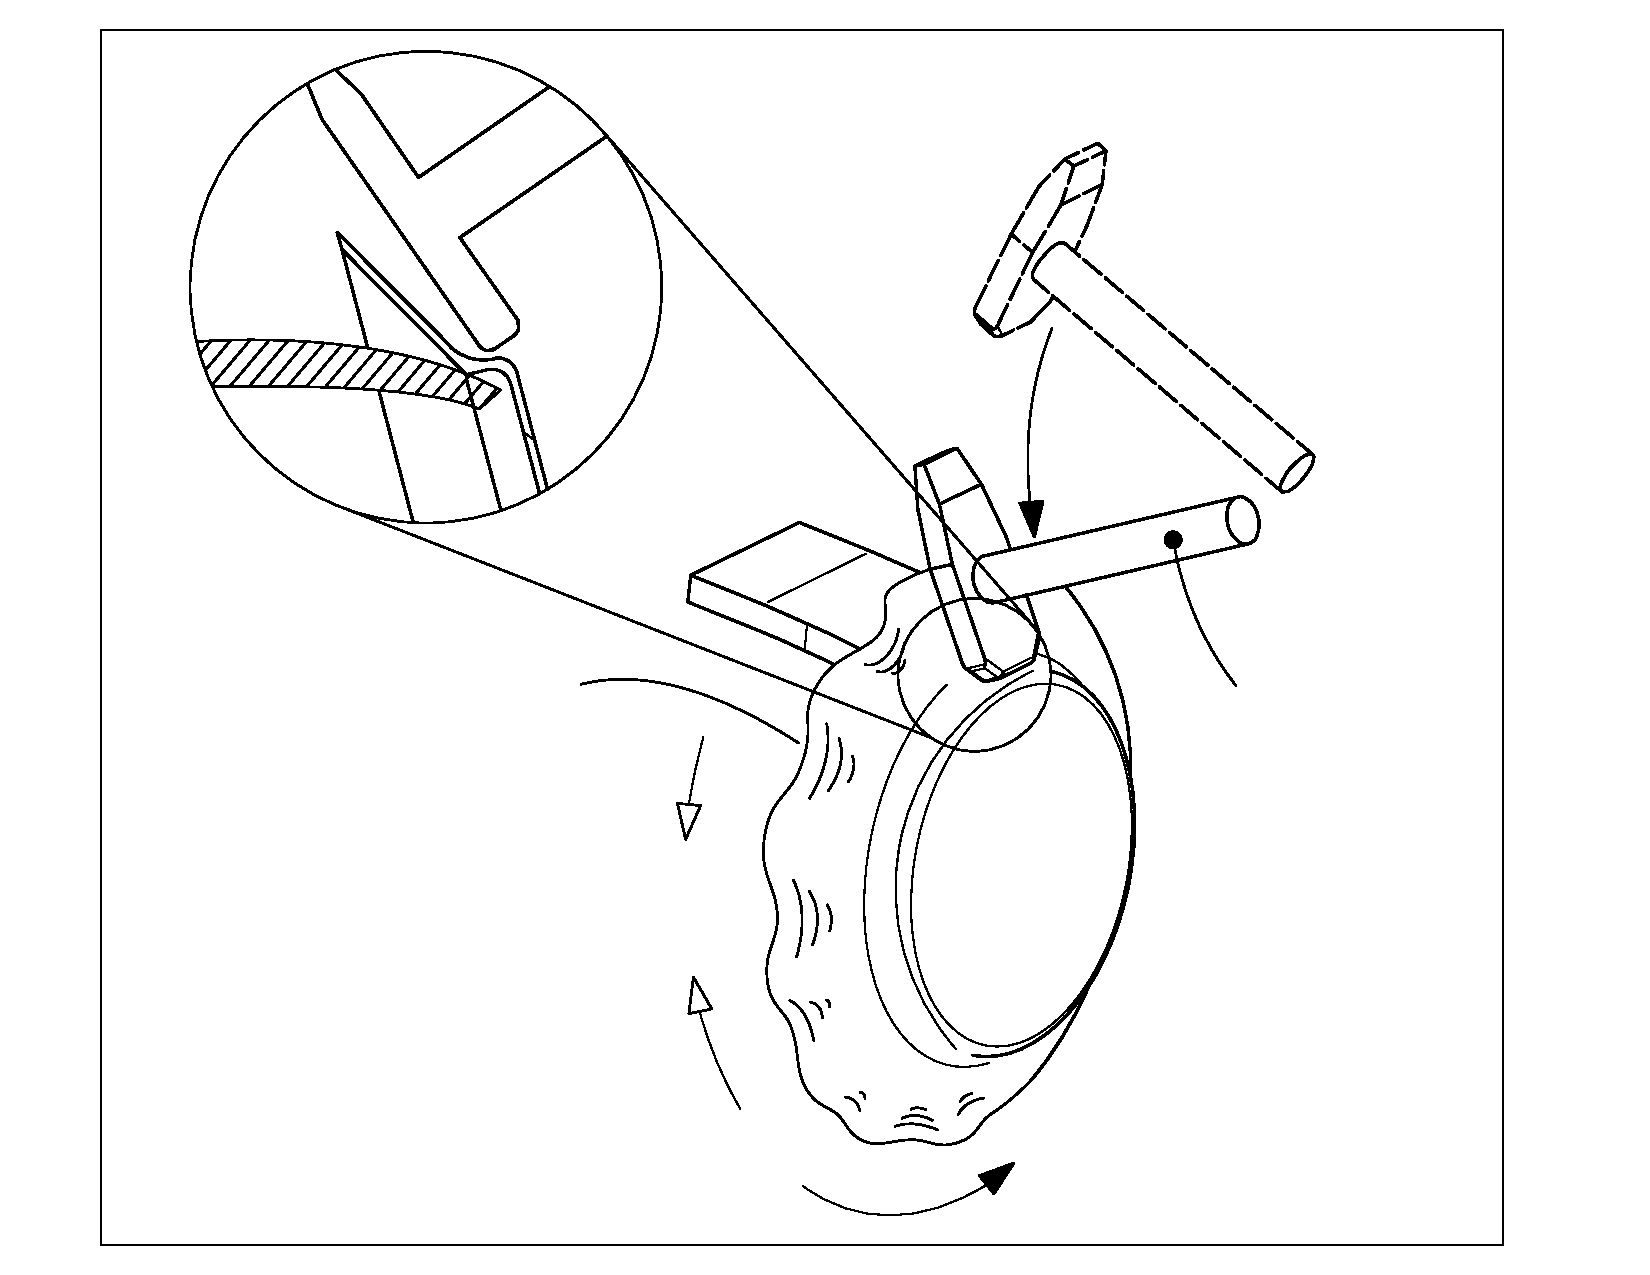
\includegraphics[trim={3cm 1cm 3cm 0.75cm },clip,width=6cm]{Images/DrawingsV3/RaisingTechDrawing.pdf}};
\node[anchor=north] at (p4) {(c)};
%
\node[] at (13.25,4) (p5) {};
\node[anchor=south] at (p5) () {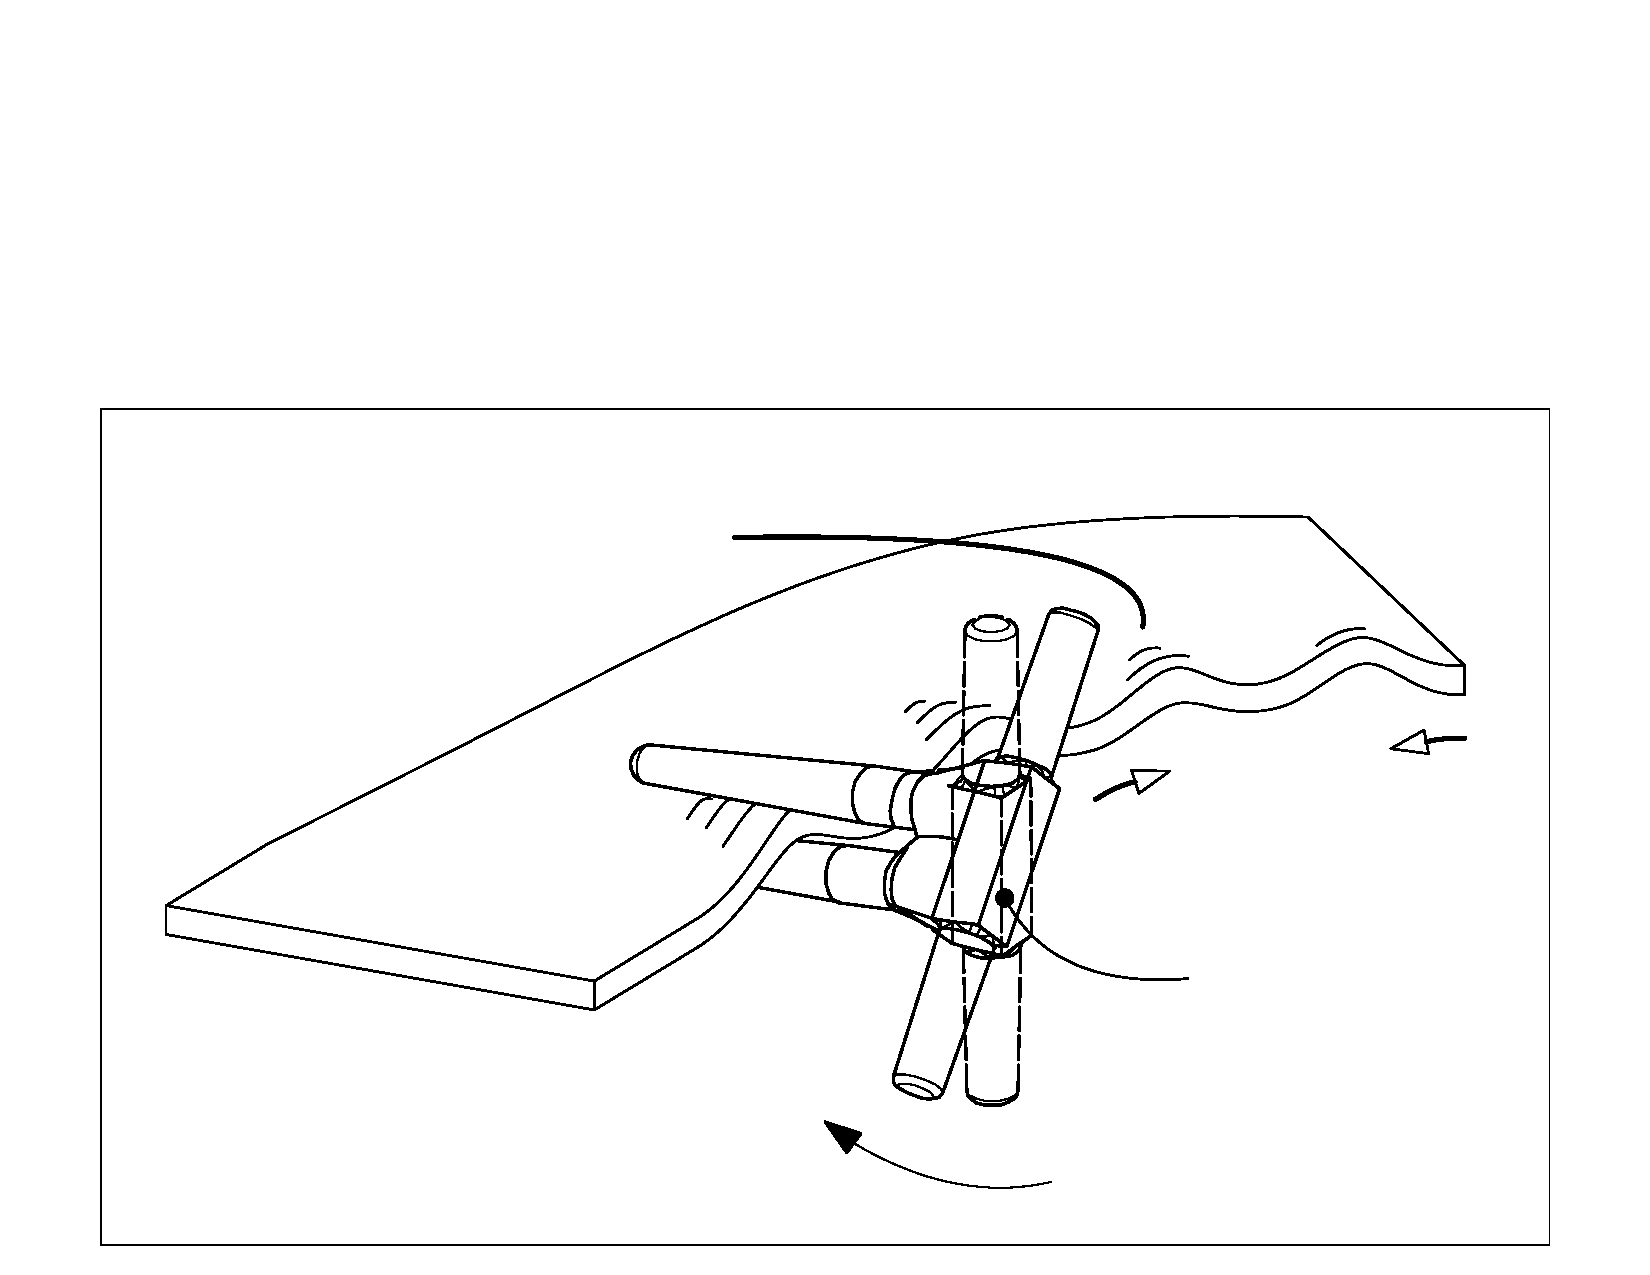
\includegraphics[trim={2cm 1cm 2cm 8cm },clip,width=8cm]{Images/DrawingsV3/TuckingTechDrawing.pdf}};
\node[anchor=north] at (p5) {(e)};
%
% %
%
{\fontfamily{\sfdefault}\selectfont 

%
\node[text width=3cm,align=right,anchor=east,xshift=-1.1cm,yshift=4.5cm] at (p1) () {Bossing \\ Mallet};
\node[text width=3cm,align=left,anchor=west,xshift=1.6cm,yshift=3cm] at (p1) () {Folding \\ Jig};
\node[text width=3cm,align=left,anchor=west,xshift=1.7cm,yshift=2cm] at (p1) () {Vice};
%
\node[text width=3cm,align=left,anchor=west,xshift=1.7cm,yshift=3.8cm] at (p2) () {Hammer \\ (Small, \\ steel head)};
\node[text width=3cm,align=left,anchor=west,xshift=2cm,yshift=1.7cm] at (p2) () {Anvil};
%
\node[text width=3cm,align=left,anchor=west,xshift=1cm,yshift=3.3cm] at (p3) () {Hammer};
\node[text width=3cm,align=left,anchor=west,xshift=1.2cm,yshift=0.8cm] at (p3) () {Thickening};
%
\node[text width=3cm,align=right,anchor=east,xshift=-0.5cm,yshift=1.5cm] at (p4) () {Shrinking \\ Circumference};
\node[text width=3cm,align=left,anchor=west,xshift=1.5cm,yshift=2cm] at (p4) () {Hammer \\ (Small, \\ steel head)};

%
\node[text width=3cm,align=right,anchor=east,xshift=-0.5cm,yshift=4cm] at (p5) () {Wrinkles};
\node[text width=3cm,align=left,anchor=west,xshift=1.9cm,yshift=2.5cm] at (p5) () {Shrinking};
\node[text width=3cm,align=left,anchor=west,xshift=2.1cm,yshift=1.5cm] at (p5) () {Two \\ Prong Fork };



}



\end{tikzpicture}
\end{document}